\subsection{What is a Netlist?}
\label{subsec:netlist}
In its most general form, a netlist is a list of every component in an electronic design paired with a list of nets they connect to. 
Depending on the abstraction level at hand, these components can be transistors, logic gates, macrocells, or increasingly higher-level modules. 
Generally, a net denotes any group of two or more interconnected components.
In an electronics context, a net can be though of as a wire connecting multiple pins between multiple components, with each wire having one voltage source and one or more voltage sinks. 
Thus, one could express the netlist as a hypergraph, nodes representing components, hyperedges representing wires connecting two or more component. 
More precisely, these hyperedges connect the ports between the components, not the components themselves, with each component exposing multiple ports. 

In FPGA context, the components are logical cells (\texttt{LUTs}, \texttt{CARRY4s}, etc.) or hierarchical cells (Verilog module instances) with pins connected together by wires. 
In Vivado, a Netlist can be synthesized as a Hierarchical or a Flattened netlist. 
Figure ~\ref{fig:hierarchical_design} shows an example a Verilog design with modules instantiated in a hierarchy. 
Figure ~\ref{fig:hier_netlist} shows the design synthesized into a hierarchical netlist with \textbf{hierarchical cells} and \textbf{leaf cells}. 
The synthesizer attempts to construct the module hierarchy as close to the module instantiation hierarchy defined by the user design entry. 
Figure ~\ref{fig:flat_netlist} shows the same design but synthesized into a flattened netlist. 

In either synthesized netlist, the \textbf{leaf cells}, (deepest level cells), must necessarily consist only of \textbf{primitive cells} from the architecture's primitive cell library (\texttt{LUT6}, \texttt{FDRE}, \texttt{CARRY4}, \texttt{DSP48E1}, etc.). 
The netlist can be compiled and exported as a purely structural low-level Verilog file, or an Electrinic Design Interchange Format (EDIF) file, both describing the netlist explicitly as a list of logical cells connected by a list of wires. 

\newpage
\end{multicols}
{
    \raggedright
    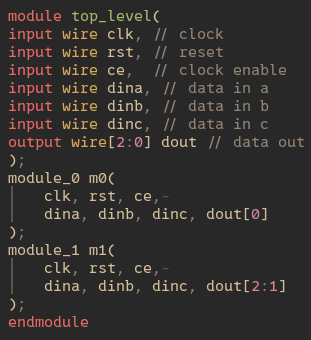
\includegraphics[valign=t, scale=0.3]{figures/netlist_synth/top_level.png}
    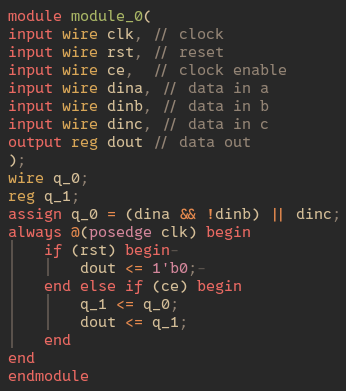
\includegraphics[valign=t, scale=0.3]{figures/netlist_synth/module_0.png}
    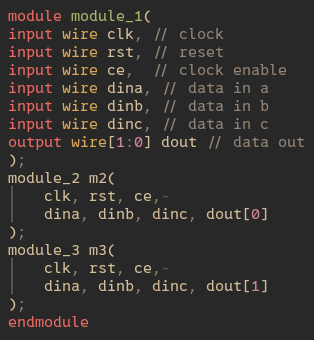
\includegraphics[valign=t, scale=0.3]{figures/netlist_synth/module_1.png}
    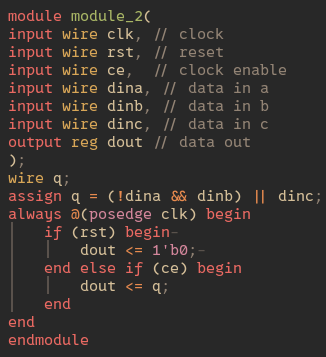
\includegraphics[valign=t, scale=0.3]{figures/netlist_synth/module_2.png}
    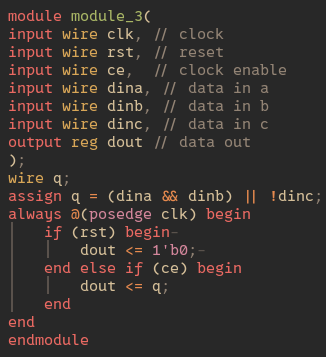
\includegraphics[valign=t, scale=0.3]{figures/netlist_synth/module_3.png}
    \captionof{figure}{A simple HDL design with module hierarchy.}
    \label{fig:hierarchical_design}
}
\vspace{0.5cm}
{
    \centering
    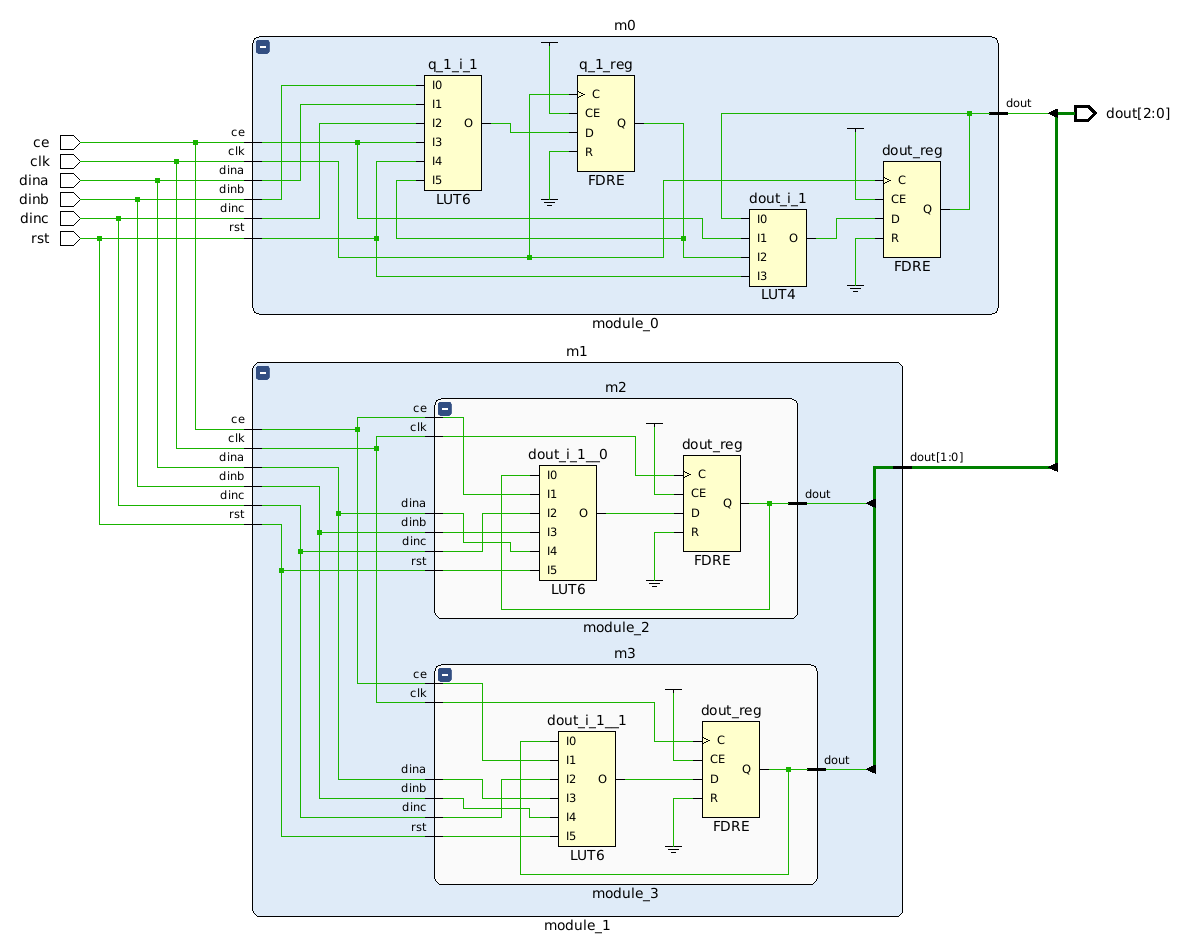
\includegraphics[valign=c, width=11.5cm]{figures/netlist_synth/hier_netlist.png}
    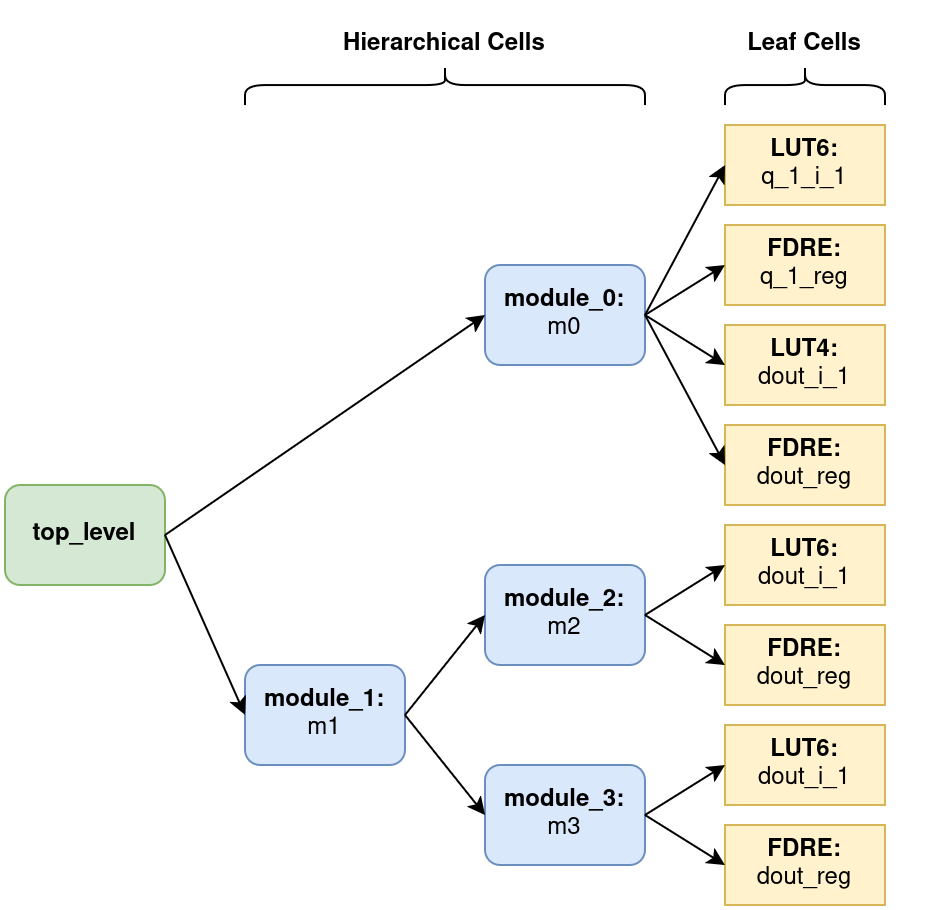
\includegraphics[valign=c, width=6cm]{figures/netlist_synth/hier_graph.png}
    \captionof{figure}{
        \textbf{Left:} A hierarchical netlist consisting of LUTs and FFs.
        \textbf{Right:} The cell hierarchy tree.
    }
    \label{fig:hier_netlist}
}
\vspace{0.5cm}
{
    \centering
    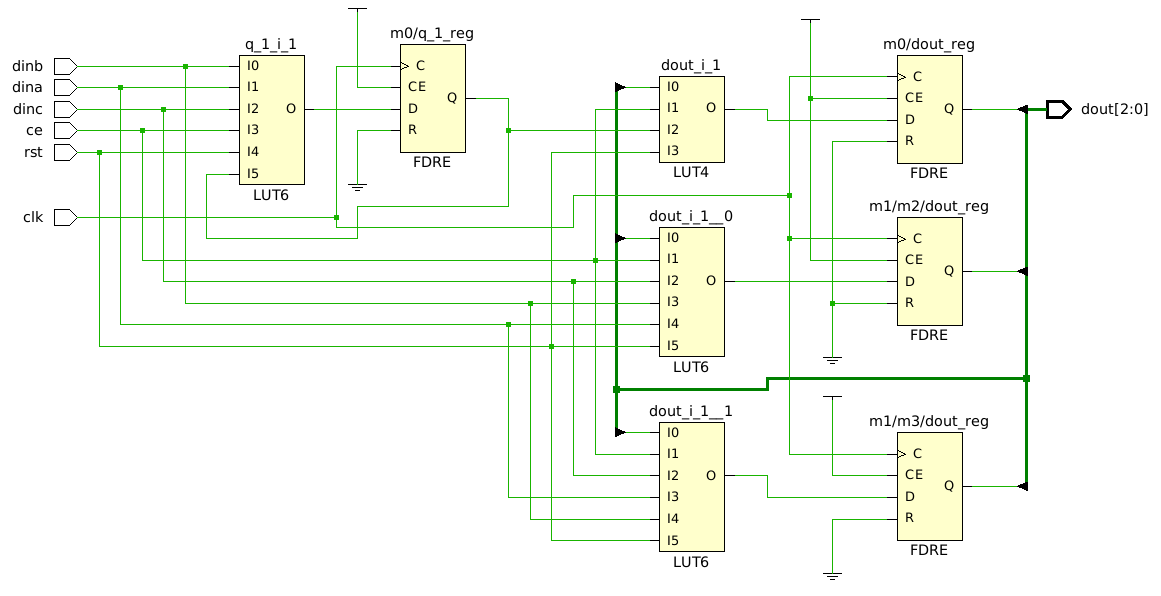
\includegraphics[valign=c, width=13.0cm]{figures/netlist_synth/flat_netlist.png}
    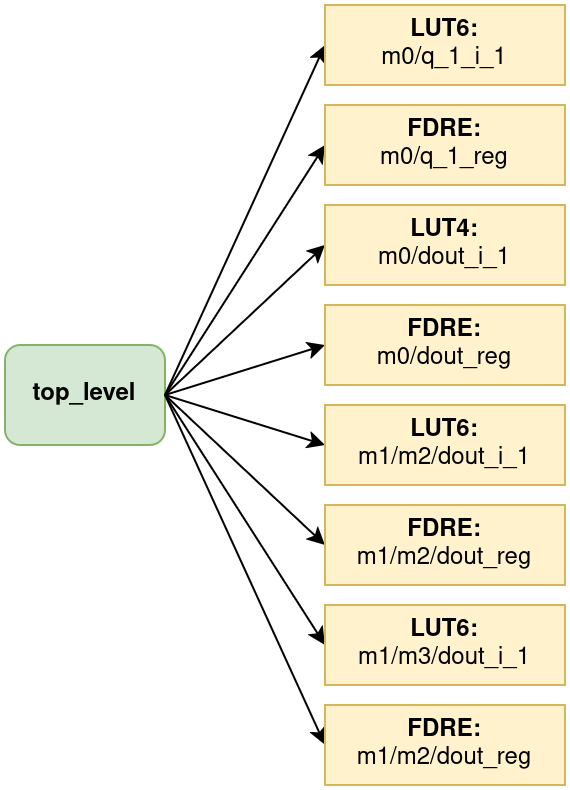
\includegraphics[valign=c, width=4cm]{figures/netlist_synth/flat_graph.png}
    \captionof{figure}{
        \textbf{Left:} A flattened netlist consisting of LUTs and FFs.
        \textbf{Right:} The flattened cell hierarchy tree.
    }
    \label{fig:flat_netlist}
}
\newpage
\begin{multicols}{2}

\subsection{Netlist Traversal and Manipulation in RapidWright}

RapidWright represents the logical netlist objects via the \texttt{edif} classes:
\begin{itemize}
    \item \texttt{EDIFNetlist}: The full logical netlist of a \texttt{Design}. 
    \item \texttt{EDIFNet}: Represents a logical net within an \texttt{EDIFNetlist}.
    \item \texttt{EDIFHierNet}: Combines an \texttt{EDIFNet} with a full hierarchical instance name to uniquely identify a net in a netlist.
    \item \texttt{EDIFCell}: Represents a logical cell in an \texttt{EDIFNetlist}. 
    \item \texttt{EDIFCellInst}: Represents an instance of an \texttt{EDIFCell}. 
    \item \texttt{EDIFHierCellInst}: An \texttt{EDIFCellInst} with its hierarchy, described by all the \texttt{EDIFCellInst}s that sit above it within the netlist.
    \item \texttt{EDIFPort}: Represents a port on an \texttt{EDIFCell}. 
    \item \texttt{EDIFPortInst}: Represents an instance of a port on an \texttt{EDIFCellInst}. 
    \item \texttt{EDIFHierPortInst}: Combines an \texttt{EDIFPortInst} with a full hierarchical instance name to uniquely identify a port instance in a netlist. 
\end{itemize}


Using these classes and their associated methods, we can traverse the logical netlist (\texttt{EDIFNetlist}) and analyze or manipulate it as we see fit. 
A netlist can be easily extracted from a \texttt{.dcp} design checkpoint file and traversed like the following example:

\begin{lstlisting}[language=java, caption={Netlist extraction and traversal}, label={lst:netlist_extract}]
Design design = Design.readCheckpoint("synth.dcp")
EDIFNetlist netlist = design.getNetlist();

// Example task:
// Extract the set of all unique nets from the design.

// Initialize a new Set:
Set<EDIFNet> netSet = new HashSet<>();

// Access all leaf cells
List<EDIFCellInst> ecis = netlist.getAllLeafCellInstances();

// Traverse the cell list
for (EDIFCellInst eci : ecis) {
    // Access the ports on this cell
    Collection<EDIFPortInst> epis = eci.getPortInsts();
    for (EDIFPortInst epi : epis) {
        // Access the net on this port
        EDIFNet net = epi.getNet();
        netSet.add(net);
    }
}

// Downstream task:
// For each unique net, print out the connected cells.

// Traverse the set of nets
for (EDIFNet net : netSet) {
    System.out.println("Net: " + net.getName());
    // Access the ports connected to this net
    Collection<EDIFPortInst> epis = net.getPortInsts();
    for (EDIFPortInst epi : epis) {
        // Access the cell that this port belongs to
        EDIFCellInst eci = epi.getCellInst();
        if (eci == null) {
            // (top_level ports have no associated cell)
            continue;
        } else {
            System.out.println(
                "\tCell: " + eci.getName() + 
                ",\tCellType: " + eci.getCellName()
            );
        }
    }
}
\end{lstlisting}

{
    \centering
    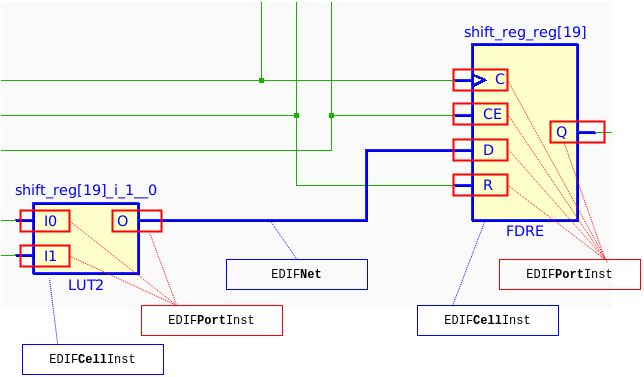
\includegraphics[valign=c, width=\columnwidth]{figures/traversal.png}
    \captionof{figure}{\texttt{Netlist} traversal via the \texttt{EDIFCellInst}, \texttt{EDIFPortInst}, and \texttt{EDIFNet} classes}
    \label{fig:traversal}
}
\vspace{0.5cm}

\begin{lstlisting}[caption={Code Printout}]
Net: dout[0]
	Port: I0, Cell: dout_i_1, CellType: LUT4
	Port: Q, Cell: m0/dout_reg, CellType: FDRE
Net: q_1
	Port: I2, Cell: dout_i_1, CellType: LUT4
	Port: Q, Cell: m0/q_1_reg, CellType: FDRE
	Port: I5, Cell: q_1_i_1, CellType: LUT6
Net: ce
	Port: I1, Cell: dout_i_1, CellType: LUT4
	Port: I1, Cell: dout_i_1__0, CellType: LUT6
	Port: I1, Cell: dout_i_1__1, CellType: LUT6
	Port: I3, Cell: q_1_i_1, CellType: LUT6
Net: dout[1]
	Port: I0, Cell: dout_i_1__0, CellType: LUT6
	Port: Q, Cell: m1/m2/dout_reg, CellType: FDRE
Net: dout_i_1__1_n_0
	Port: O, Cell: dout_i_1__1, CellType: LUT6
	Port: D, Cell: m1/m3/dout_reg, CellType: FDRE
Net: clk
	Port: C, Cell: m0/dout_reg, CellType: FDRE
	Port: C, Cell: m0/q_1_reg, CellType: FDRE
	Port: C, Cell: m1/m2/dout_reg, CellType: FDRE
	Port: C, Cell: m1/m3/dout_reg, CellType: FDRE
Net: dout[2]
	Port: I0, Cell: dout_i_1__1, CellType: LUT6
	Port: Q, Cell: m1/m3/dout_reg, CellType: FDRE
Net: <const0>
	Port: G, Cell: GND, CellType: GND
	Port: R, Cell: m0/dout_reg, CellType: FDRE
	Port: R, Cell: m0/q_1_reg, CellType: FDRE
	Port: R, Cell: m1/m2/dout_reg, CellType: FDRE
	Port: R, Cell: m1/m3/dout_reg, CellType: FDRE
Net: <const1>
	Port: P, Cell: VCC, CellType: VCC
	Port: CE, Cell: m0/dout_reg, CellType: FDRE
	Port: CE, Cell: m0/q_1_reg, CellType: FDRE
	Port: CE, Cell: m1/m2/dout_reg, CellType: FDRE
	Port: CE, Cell: m1/m3/dout_reg, CellType: FDRE
Net: dout_i_1__0_n_0
	Port: O, Cell: dout_i_1__0, CellType: LUT6
	Port: D, Cell: m1/m2/dout_reg, CellType: FDRE
Net: rst
	Port: I3, Cell: dout_i_1, CellType: LUT4
	Port: I5, Cell: dout_i_1__0, CellType: LUT6
	Port: I5, Cell: dout_i_1__1, CellType: LUT6
	Port: I4, Cell: q_1_i_1, CellType: LUT6
Net: dinc
	Port: I2, Cell: dout_i_1__0, CellType: LUT6
	Port: I2, Cell: dout_i_1__1, CellType: LUT6
	Port: I2, Cell: q_1_i_1, CellType: LUT6
Net: dinb
	Port: I3, Cell: dout_i_1__0, CellType: LUT6
	Port: I4, Cell: dout_i_1__1, CellType: LUT6
	Port: I0, Cell: q_1_i_1, CellType: LUT6
Net: dina
	Port: I4, Cell: dout_i_1__0, CellType: LUT6
	Port: I3, Cell: dout_i_1__1, CellType: LUT6
	Port: I1, Cell: q_1_i_1, CellType: LUT6
Net: q_1_i_1_n_0
	Port: D, Cell: m0/q_1_reg, CellType: FDRE
	Port: O, Cell: q_1_i_1, CellType: LUT6
Net: dout_i_1_n_0
	Port: O, Cell: dout_i_1, CellType: LUT4
	Port: D, Cell: m0/dout_reg, CellType: FDRE
\end{lstlisting}





